% !TEX root = ../main.tex

% = = = = = = = = = = = = = = = = = = = = = = = = = = = = = = = = = = = = = = = = = = = = = = %
%
%
%
%
%
%
% = = = = = = = = = = = = = = = = = = = = = = = = = = = = = = = = = = = = = = = = = = = = = = %

\section{Threat Model}

The attack surface to abuse users' browsers through cryptojacking is broad, and there are multiple vectors where various entities can inject mining scripts in the website's codebase. We summarize those here. 

\subsection{Webmaster initiated} 

A website administrator can add a mining script to her webpage, with or without informing users. Website owners may do this to monetize their sites, especially when they have been blacklisted or blocked by standard advertising platforms. In one example, a researcher found Coinhive on a large Russian website offering child pornography to users~\cite{coinhiveonchildporn}. Revenue estimates, based on the website traffic data available, were roughly \$10,000 a month after converting the value of XMR mined to USD.

\subsection{Mixed content} 

Many websites serve active Javascript from third parties within their own webpages. This could be ads from an ad network or tools for tracing users of their site. Third parties with these privileges can inject cryptojacking scripts into the sites that use them. In two separate incidents, Coinhive was injected into the websites of Movistar\footnote{Movistar is a major telecommunications brand owned by Telefonica, operating in Spain and in many Hispanic American countries \url{https://www.movistar.com/}} and Globovision\footnote{Globovision is a 24-hour television news network in Venezuela and Latin America \url{http://globovision.com/}} using Google Tag Manager\footnote{Google Tag Manager is a tag management system created by Google to manage JavaScript and HTML tags used for tracking and analytics on websites}. Movistar stated that Coinhive was not put on their website by a hacker, but instead was due to \textit{``internal error''} while they were conducting ``production tests.'' No statement was provided by Globovision on why the cryptojacking scripts appeared on their site on November 15, 2017~\cite{googletagcoinhive}.

\subsection{Browser extensions} 

Cryptojacking was not limited to websites in 2017. The Chrome extension Archive Poster remained on the Chrome Web Store for days while silently cryptojacking an unknown portion of their 100,000+ users. After multiple user reports, followed by multiple news media outlets covering the issue, the extension was removed~\cite{chromeextentioncoinhive}. 

\subsection{Breaches} 


If an attackers is able to breach principle servers, websites, extensions, or the scripting services they use, they can inject cryptojacking scripts that will impact the site's users without the site's knowledge or consent. For example, a researcher found a malicious modification to webchat system LiveHelpNow's SDK; it resulted in unsolicited mining across all websites using their char support service~\cite{chatsupporthack}. In another example, Coinhive was found on the political fact-checking website PolitiFact\footnote{PolitiFact: Fact-checking US politics.\url{https://politifact.com/}} A compromised JavaScript library was found to be injecting the cryptojacking scripts. The malicious code remained on the site for at least four hours before it was removed~\cite{politifactcoinhive}. PolitiFact executive director stated, ``Hackers were able to install their script on the fact-checking website after discovering a misconfigured cloud-computing server''~\cite{politifactcoinhivewsj}.


\subsection{Man-in-the-middle} 

A user's web traffic is often routed through intermediaries that may have plaintext access to content. For example, internet service providers or free public wireless routers can inject cryptojacking scripts into non-HTTPS traffic. Advertisement code injection has been seen in practice ~\cite{vergeadinjection}. There have been assertions of similar injections of browser mining scripts at certain Starbucks free Wi-Fi hotspots\footnote{\url{https://twitter.com/imnoah/status/936948776119537665}}.






% = = = = = = = = = = = = = = = = = = = = = = = = = = = = = = = = = = = = = = = = = = = = = = %
%
%
%
%
%
%
% = = = = = = = = = = = = = = = = = = = = = = = = = = = = = = = = = = = = = = = = = = = = = = %

\section{Measurements}

\subsection{Prevalence of Coinhive and alternatives}

\begin{figure}[t]
\begin{tabular}{c}
\begin{lstlisting}[language=sql]
SELECT domain, tags, p80.http_www.get.headers.content_language, p80.http_www.get.headers.server, p80.http.get.headers.x_powered_by, p80.http.get.title, p80.http_www.get.body as wwwbody, p80.http.get.body as plainbody 
FROM censys-io.domain_public.20171123
WHERE STRPOS(p80.http.get.body, coinhive.min.js) > 0 or STRPOS(p80.http_www.get.body, coinhive.min.js) >0)
\end{lstlisting}
\end{tabular}
\caption{A BigQuery SQL query to find websites that embed the Coinhive script using a dataset of the top one million sites from censys.io. \label{lst:bigquery}}
\end{figure}

\begin{figure}[t]
\centering
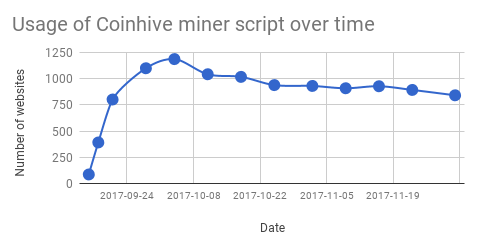
\includegraphics[width=\linewidth]{figures/usage_of_coinhive_over_time.png}
\caption{The number of instances of the Coinhive miner scripts found using the query in Figure~\ref{lst:bigquery} in top one million websites over a three month period beginning with the release of Coinhive in September 2017.\label{fig:topmil}}
\end{figure}

Based on the fact that Coinhive is the dominant website offering in-browser mining, See Figure~\ref{fig:coinhivevscopycats}, we focus on measuring the prevalence of Coinhive scripts deployed on internet sites. We use the censys.io BigQuery dataset ~\cite{censys15} for the top million sites indexed by Zmap\footnote{\url{https://zmap.io}}. We simply look for the \texttt{coinhive.min.js} script within the body of the website page. The query we use is in Figure~\ref{lst:bigquery} and the results over a two month period are provided in Figure~\ref{fig:topmil}. These findings are corroborated by another search engine, PublicWWW, which indexes the source code of publicly available websites. Using PublicWWW's dataset, over 30,000 websites were found to have the \texttt{coinhive.min.js} library.\footnote{Citation to blog post detailing our results removed for anonymity.} As seen from our data in Figure~\ref{fig:topmil}, the adoption of this script was substantial in the first days of its release. However, progress slowed down at the same time as ad-blockers and organizations started to block Coinhive's website. The initial purpose of this service, as claimed by Coinhive, was to replace ads and cover server costs for webmasters. As the service did not require that websites received user consent before beginning to mine, it started to be used maliciously in users` browsers. This type of usage resulted in Coinhive being included in some company's top-10 most wanted malware list~\cite{checkpoint}.

% JC: After anon, cite ~\cite{badpacketspublicwww}

This type of measurement will become less accurate moving forward. Cryptojacking services are evolving to use obfuscated JavaScript and randomized URLs to evade detection\footnote{\url{https://twitter.com/bad_packets/status/940333744035999744}}. An example of these methods can be found in the cryptojacking service provider called Minr. In this case, the script is automatically obfuscated for users implementing the code. In addition, the domain names used by Minr frequently change to circumvent blocklists and anti-malware software.

\begin{figure}[t]
\centering
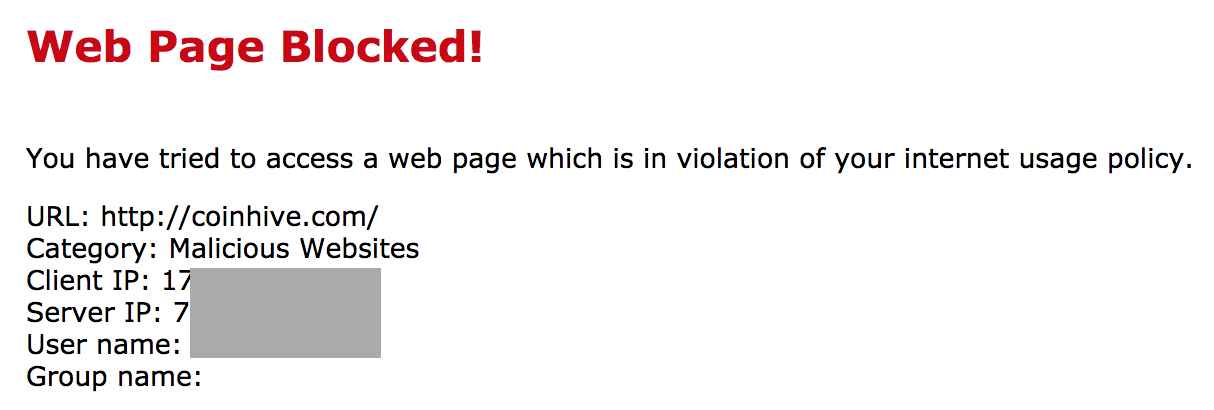
\includegraphics[width=0.9\linewidth]{figures/coinhive_blocked.png}
\caption{Our university has categorized the coinhive.com website as malicious and has blocked it.\label{fig:concordia}}
\end{figure}

\begin{table}[t]
\centering
\begin{tabular}{|cc|c|}
\hline
\textbf{Website} & \textbf{Results} & \textbf{Query Parameter}  \\ \hline
Coinhive & 30611 & `coinhive.min.js`   \\  \hline
JSEcoin & 1131 & `load.jsecoin.com`   \\  \hline
Crypto-Loot & 695 & `CryptoLoot.Anonymous`  \\  \hline
Minr & 324 & `minr.pw`,`st.kjli.fi`, \\
~  & ~ &  `abc.pema.cl`,`metrika.ron.si`, \\  
~  & ~ &  `cdn.rove.cl`,`host.d-ns.ga`, \\  
~  & ~ &  `static.hk.rs`,`hallaert.online`, \\  
~  & ~ &  `cnt.statistic.date`,`cdn.static-cnt.bid` \\     \hline
CoinImp & 317 &`www.coinimp.com/scripts/min.js`,  \\  \hline
~  & ~ &  `www.hashing.win` \\     \hline
ProjectPoi (PPoi) & 116 & `projectpoi.min`  \\  \hline
AFMiner & 46 & `afminer.com/code/miner.php`	  \\  \hline
Papoto & 42 & `papoto.com/lib/papoto.js`  \\ \hline
\end{tabular}
\caption{Cryptojacking data was gathered by totalling the number of websites which had the following libraries in their source codes, indexed by PublicWWW by 12/24/2017. Figure~\ref{fig:coinhivevscopycats} and Figure~\ref{fig:copycat} are visualizations of these result.\label{tab:findcoinhive}}
\end{table}

\begin{figure}[t]
\centering
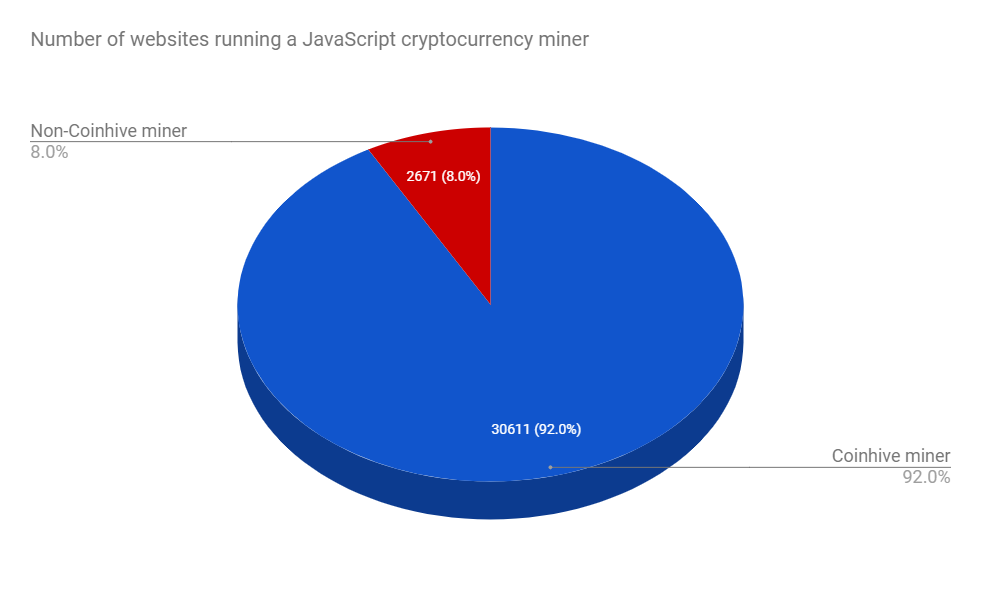
\includegraphics[width=0.9\linewidth]{figures/coinhive-miners-pie.png}
\caption{Share of websites using a Javascript cryptocurrency miner, details in Table~\ref{tab:findcoinhive}  \label{fig:coinhivevscopycats}}
\end{figure}

\begin{figure}[t]
\centering
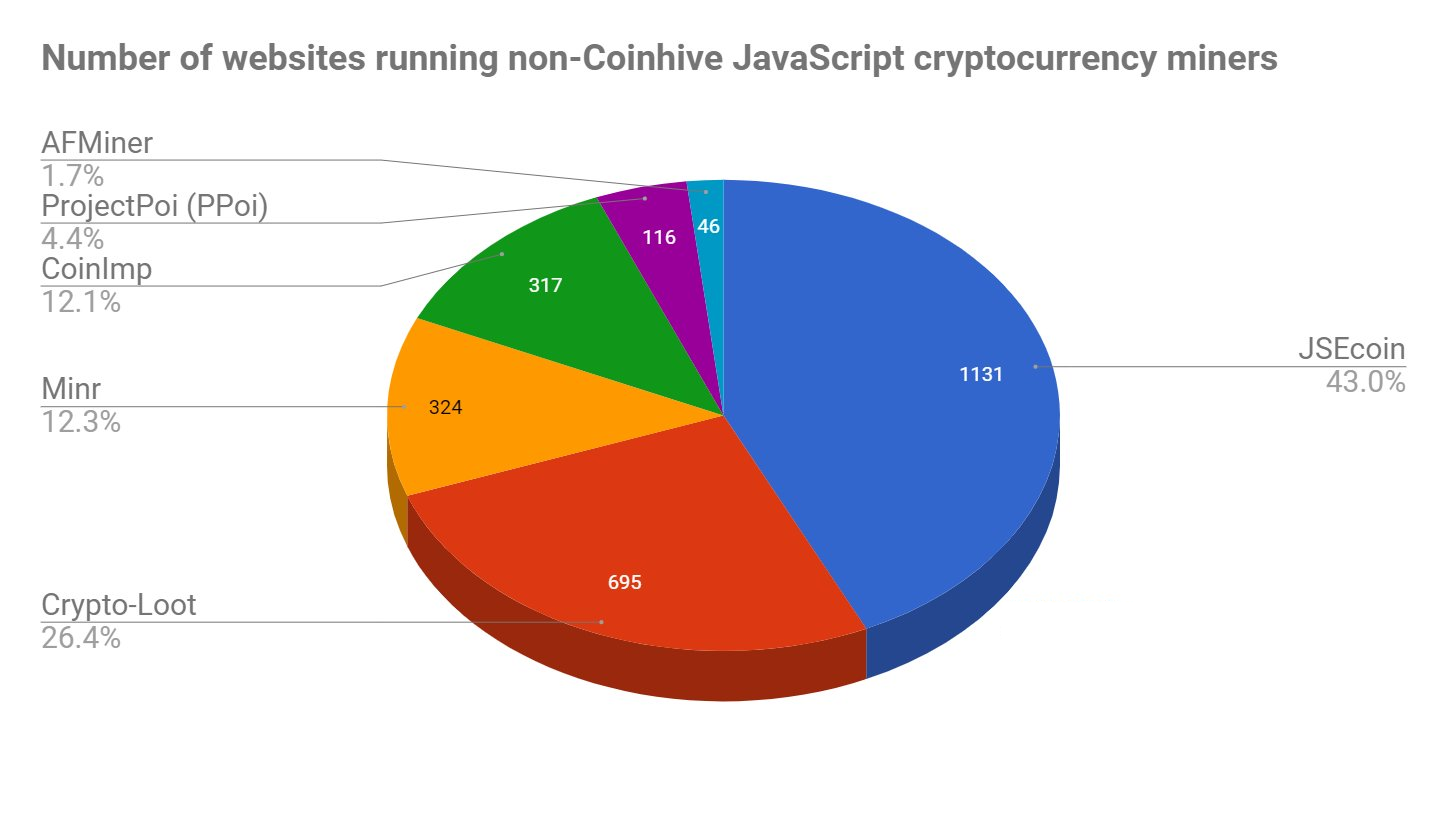
\includegraphics[width=0.9\linewidth]{figures/non-coinhive-miners-pie.png}
\caption{Share of websites using a Coinhive alternatives, details in Table~\ref{tab:findcoinhive}  \label{fig:copycat}}
\end{figure}

\begin{figure}[t]
\centering
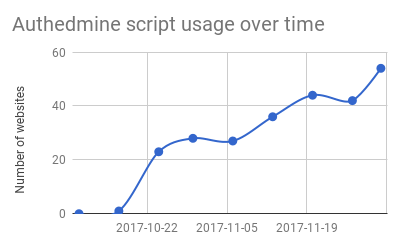
\includegraphics[width=0.9\linewidth]{figures/usage_of_authedmine_over_time.png}
	\caption{Usage of AuthedMine Miner scripts in top one million websites since its introduction.\label{fig:authmine}}
\end{figure}

\begin{figure}[t]
\centering
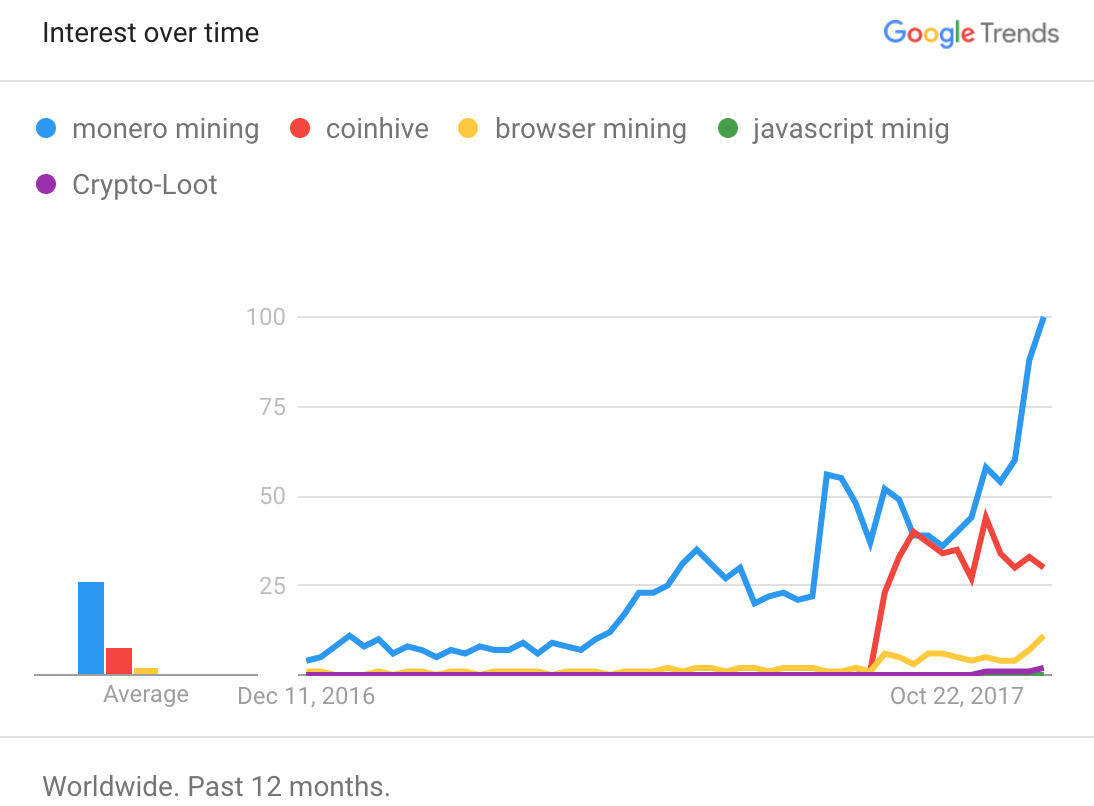
\includegraphics[width=0.9\linewidth]{figures/usage_over_time2.png}
\caption{Google Trend over last 12 months: there has been more interest in Coinhive than the broader, related search term ``Browser mining''. Comparing to other services offering Monero browser mining API, Coinhive had the advantage of being the first to offer the service. \label{fig:trend}}
\end{figure}



Coinhive has begun to be blocked by enterprises. One example is shown in Figure~\ref{fig:concordia}. This blocking seems to have sent Coinhive operators to lesser known alternatives with the same or similar functionality. We used the same methodology on another dataset, PublicWWW\footnote{Search Engine for Source Code \url{https://publicwww.com/}} to find the usage of Coinhive and its alternatives the internet. Table~\ref{tab:findcoinhive} shows the keywords used to identify these services. The result can be found on Figure~\ref{fig:coinhivevscopycats} and Figure~\ref{fig:copycat}.

Coinhive has also reacted by focusing on adding user consent and legitimizing the use of cryptojacking. It introduced another domain and service called \textit{Authedmine}, which requires user's consent to start mining in the browser. This service did not get the same attention as the original service, but it did inspire discussions regarding the ethics of such services, which is discussed in Section~\ref{sec:ethics}. Using the same methodology, censys.io was used to measure the prevalence of AuthedMine and show the results in Figure~\ref{fig:authmine}. 

\subsection{Client impact}

\begin{figure}[t]
\centering
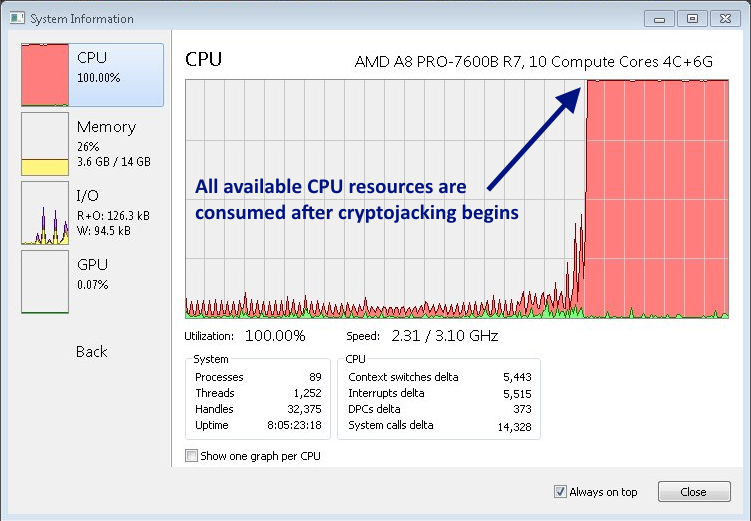
\includegraphics[width=\linewidth]{figures/windows_cpu_usage.png}
	\caption{Comparison of CPU usage of browser without and with browser mining enabled.}\label{fig:cpu}
\end{figure}

Most cryptojacking scripts discovered were configured to use around 25\% of user's CPU, which can be justified as it will be under the threshold of attracting the user's attention, and it could be argued as fair-usage of their hardware. During the first few days, however, there were some reports of 100\% CPU usage when visiting websites containing these scripts~\cite{piratesbayblog}, which can be characterized as malicious. By default, the Coinhive JavaScript library will use all available CPU resources available. The user implementing the script must include a throttle value to reduce the client-side CPU usage during mining operations. We show an example in Figure~\ref{fig:cpu}.


\subsection{Profitability}
\label{profitabilitexperiment}

\begin{figure}[t]
\centering
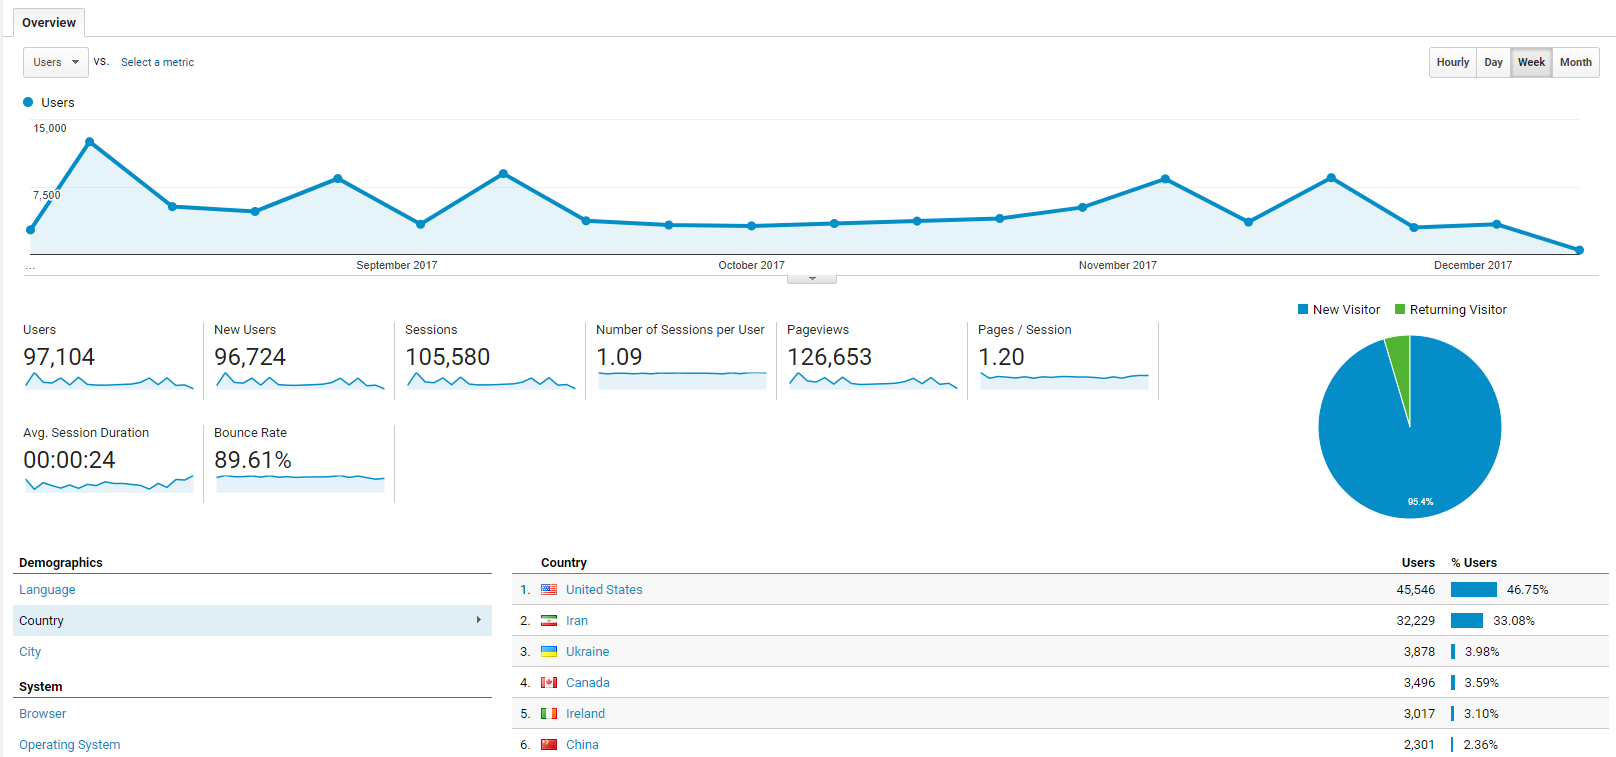
\includegraphics[width=\linewidth]{figures/experiment_analytics_results.png}
\caption{Google Analytics dashboard showing the number of visitors to a domain parking service of 11\,000 domains.}\label{fig:domain2}
\end{figure}

\begin{figure}[t]
\centering
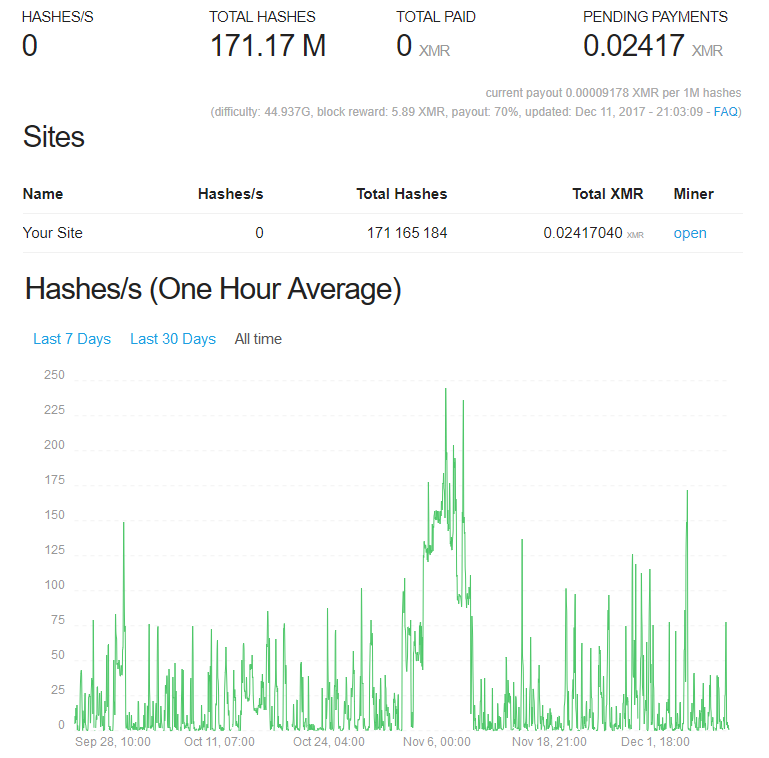
\includegraphics[width=\linewidth]{figures/experiment_coinhive_results.png}
\caption{Coinhive dashboard showing the earnings of a domain parking service that runs Coinhive on 11\,000 domains. Over the course of about 3 months, the operator earned 0.02417 XMR (currently \$7.69 USD).}\label{fig:domain1}
\end{figure}

Coinhive developers estimate a monthly revenue of about 0.3 XMR (about \$101 USD) for a website with 10-20 active miners~\cite{coinhive}. We sought to validate this estimation with a real world data set provided to us\footnote{In collaboration and with thanks to Faraz Fallahi: \url{https://github.com/fffaraz}}. One of the biggest Coinhive campaign operators is a domain parking service. It runs Coinhive on over 11\,000 parked websites. While visits to parked domains are considerably shorter than an average website, the data spans a period of three months and gives some insight into the profitability of cryptojacking. During the experimental period of about 3 months, they accumulated 105\,580 user sessions for an average of 24 seconds per session. For the period examined, the revenue was 0.02417 XMR (Monero's currency) which at the time of writing is valued at \$7.69 USD. Further detail is provide in Figures~\ref{fig:domain2} and \ref{fig:domain1}. While an A/B test was not setup to determine how much traditional web advertising would have brought in, freely available web calculator tools suggest we might expect an order or two of magnitude greater for comparable traffic. 


% = = = = = = = = = = = = = = = = = = = = = = = = = = = = = = = = = = = = = = = = = = = = = = %




\section{Mitigations}

We discuss the ethics of cryptojacking in the next section, but in the case of cryptojacking without user consent, it is seems natural to us to presuppose users want to be protected. Protection might take a few forms, which we outline here.

\subsection{Obtaining consent}

Cryptojacking tools might attempt to legitimize the practice by first obtaining user consent on a service provider level. An example of this is the Authedmine service from Coinhive discussed previously. Malicious sites might also opt for a service like Authedmine if it is whitelisted on its users` networks and then attempt to circumvent the consent process. For example, consent that requires a click from the user has been shown in some circumstances to be vulnerable to clickjacking attacks~\cite{rydstedt2010busting}.

While cryptojacking is nowhere near the prevalence of tracking cookies, eventually it might grow into regulatory issues where governmental bodies could use legislative approaches to obtain consent, similar to the provisions many countries now use for cookies (including honouring the `do not track' HTTP header and obtaining click-based consent).

%In addition to regulation and standardizing, better security design is required to narrow down the attack surface, such as using SSL/TLS and tokenizing the requests to make sure websites get user`s consent before running these scripts. DNS TXT records could also be implemented to verify domain name ownership before browser mining scripts would be authorized to run on the website.

\subsection{Browser-level mitigation}

Browser developers have begun discussion of intervening in cryptojacking\footnote{`Please consider intervention for high cpu usage js' \url{https://bugs.chromium.org/p/chromium/issues/detail?id=766068}}~\cite{operanocoin}. Potential mitigations include: throttling clientside scripting, warning users when clientside scripting consumes excessive resources, and blocking the sources of known cryptojacking scripts. Determining appropriate for thresholds for client-side processing that are high enough to allow legitimate applications and low enough to deter cryptojacking is an open problem, as would be the wording of any notifications to the user that would lead the user to make an informed decision about allowing or not allowing resource consumption (\cf SSL/TLS warnings~\cite{SEAAC09,SHB11,Acer:2017:WWR:3133956.3134007}).
Browsers such as Opera, have taken a stance against cryptojacking scripts and blocked them via "NoCoin" blacklist ~\cite{operanocoin}. The effectiveness of using a blacklist to block such activities is still not clear. %maybe a bit more on this? meaning that as seen so far, cryptojackers can just use new domains/ips to bypass these blacklists

It is worth noting that browsers might actually take the exact opposite approach and promote (consensual) in-browser mining. This new model of monetizing websites can be a paradigm shift in how advertisement giants monopolize internet traffic. This could lead to re-democratizing the online advertisement ecosystem to make it fairer for smaller players. Browser mining has been shown to not be as efficient as native mining applications today. Therefore, optimizations on how browsers pass system calls to the operating system can be made, or there can even be browsers designed specifically to support efficient browser mining. 


% = = = = = = = = = = = = = = = = = = = = = = = = = = = = = = = = = = = = = = = = = = = = = = %

\section{Ethical Considerations}
\label{sec:ethics}

The opinion of the authors of this paper maintain that users should be given the option to enable the miner code in their browser only with some benefit to their experience on the website. Recent polls support this notion, such as the one conducted by Bleeping Computer, which found that ``many users said they are OK with websites mining Monero in the background if they don`t see ads anymore''~\cite{bleepingcomputerminers}. Another example would be granting access to premium features of the website such as journal articles behind a paywall, or streaming in high-definition. The website could also allow the user to participate in mining rewards by allocating a large portion of their CPU resources to the activity of mining, which would benefit both parties. By notifying the user of the potentials of such activity, and allowing them to make a choice to participate, the website maintains trust in their relationship with the user while also benefiting from a new source of revenue. By foregoing disclaiming this new activity, which can have harmful effects, the website will gain a new revenue stream for a short time only while sacrificing their reputation in the long term. Coinhive`s recent response to the market`s negative reaction by releasing AuthedMine, which enforces user consent before enabling any mining JavaScript code, justifies this rationale. However, before consented browser mining could develop into a sustainable model, its security implications and user impact should be addressed.

Replacement of online advertisement with in-browser mining could be a new way to monetize website`s traffic. However this will result in a paradigm shift in website monetization. As an example in both auction-based and keyword-based online advertisement, the advertiser pays the advertisement publisher to distribute the advertisment and the advertisement publisher pays a portion of the revenues to the website owner whom the advertisement was shown on her website~\cite{king2007internet}. However in in-browser mining as a replacement monetization strategy, user is technically paying for their website visit on their electricity bill, in which the consent of the user becomes an ethical issue. 

As the concept of website traffic revenue begins to change, the values associated with the old concept will have to be reexamined. Moor, in "What is Computer Ethics?" ~\cite{moor1985computer} introduces the concept of \textit{Invisible Factor}, for invisible computer operations in society. Based on his definitions cryptojacking falls under \textit{Invisible abuse}, the intentional use of the invisible operations of a computer to engage in unethical conduct. Here the cryptojacker is earning money from unaware users that are being charged on their electricity bill. 

%TODO: this paragraph can be shortened. the point is the story of piratesbay and how they dealth with it
Most browser mining code is executed without the consent, nor knowledge, of the users involved. As previously mentioned, the websites that have been found running JavaScript code for the purpose of mining usually employed Coinhive`s API. One such website, for example, ThePirateBay.org~\cite{bbcmintcrypto}, which ran the JavaScript code when users searched for torrent files. Perhaps unsurprisingly, there was no notice in their Privacy Policy nor visible warning on any part of the website that informed their users of this activity. This resulted in a backlash against the website, which responded with the following statement, ``Do you want ads or do you want to give away a few of your CPU cycles every time you visit the site?'' ~\cite{piratesbayblog}. While they admitted to their testing of browser mining, their notice came after the fact and resulted in the removal of the JavaScript code altogether due to upset users. This is in contrast to the banners users are presented with upon the first visit to a website that warns them of the website`s policy on cookies, which is enforced today through EU laws~\cite{eucookie}. It is now widely known that these cookies can be used to track users across the internet, so cookie banners can act as a reminder and allow the user to make better informed decisions regarding their browsing habits. Without any type of disclaimer for users, websites have been commandeering their users` CPU resources for their business and personal gain. This results in higher energy bills for the user, along with accelerated device degradation, slower system performance, and poor web experience~\cite{httparchiveminingimpact}\cite{gaurdianelectricity}.


%TODO: the next two paraphraphs also has been talked about before. can combine both together.
A second example of a popular website deploying Coinhive`s API is Showtime.com, which is a popular cable channel that also streams their TV shows online. Showtime has declined to comment on how or why Coinhive was implemented on their website. Speculation has been raised that it was injected via an third-party analytics tool, New Relic, due to Coinhive being found inside the New Relic code block within showtime`s website source code. However a New Relic representative denied these claims in a statement to The Register, "It appears they [Coinhive scripts] were added to the website by its [Showtime's] developers." ~\cite{registershowtime}. 
It was then hardly surprising when UFC.com was accused of using this very same code on the night of streaming one of their most popular events~\cite{registerufcmonero}. In a statement released by the UFC, they denied the presence of the code stating, ``[they] did not find any reference to the mentioned Coinhive JavaScript [code]``\footnote{\url{https://twitter.com/bad_packets/status/928044219222048769}}.
 
The recent trend of streaming websites deploying Coinhive's API could be due to the high costs of providing streaming services. While ads can be used to offset some of those costs, it would be of interest to some to at least experiment with the idea of recruiting their users to mine Monero for profit. This same regard is true for hackers looking to maximize their cryptojacking profits. The longer a user is engaged on a website, such as video streaming service, the more income can be earned through browser mining.

Given the recent interest some websites have shown in regard to browser mining, there is also potential for this new form of revenue generation to compete with advertisements. As seen in section~\ref{profitabilitexperiment}, an immediate impact could be to reduce how many ads a user sees on a given website. Moving forward websites with long user sessions such as streaming services could one day even replace ads. This is because the malware that is associated with advertisements is still a growing concern, and the public`s dislike of advertisements will likely persist and not wane. Also, as cryptocurrencies continue to grow in market capitalization and use cases, their inevitable mainstream use will push the profitability of mining egalitarian proof-of-work cryptocurrencies, such as Monero, well into the future. 

%The lack of regulation in cryptocurrency space allows for a grey market to grow. This is felt more when it affects non-tech-savvy users. 


% = = = = = = = = = = = = = = = = = = = = = = = = = = = = = = = = = = = = = = = = = = = = = = %


















